\documentclass[journal,12pt,twocolumn]{IEEEtran}
%
\def\inputGnumericTable{}
\usepackage{setspace}
\usepackage{gensymb}
%\doublespacing
\singlespacing

%\usepackage{graphicx}
%\usepackage{amssymb}
%\usepackage{relsize}
\usepackage[cmex10]{amsmath}
%\usepackage{amsthm}
%\interdisplaylinepenalty=2500
%\savesymbol{iint}
%\usepackage{txfonts}
%\restoresymbol{TXF}{iint}
%\usepackage{wasysym}
\usepackage{amsthm}
%\usepackage{iithtlc}
\usepackage{mathrsfs}
\usepackage{txfonts}
\usepackage{stfloats}
\usepackage{bm}
\usepackage{cite}
\usepackage{cases}
\usepackage{subfig}
%\usepackage{xtab}
\usepackage{longtable}
\usepackage{multirow}
%\usepackage{algorithm}
%\usepackage{algpseudocode}
\usepackage{enumitem}
\usepackage{mathtools}
\usepackage{steinmetz}
\usepackage{tikz}
\usepackage{circuitikz}
\usepackage{verbatim}
\usepackage{tfrupee}
\usepackage[breaklinks=true]{hyperref}
%\usepackage{stmaryrd}
\usepackage{tkz-euclide} % loads  TikZ and tkz-base
%\usetkzobj{all}
\usetikzlibrary{calc,math}
\usepackage{listings}
    \usepackage{color}                                            %%
    \usepackage{array}                                            %%
    \usepackage{longtable}                                        %%
    \usepackage{calc}                                             %%
    \usepackage{multirow}                                         %%
    \usepackage{hhline}                                           %%
    \usepackage{ifthen}                                           %%
  %optionally (for landscape tables embedded in another document): %%
    \usepackage{lscape}     
\usepackage{multicol}
\usepackage{chngcntr}
%\usepackage{enumerate}

%\usepackage{wasysym}
%\newcounter{MYtempeqncnt}
\DeclareMathOperator*{\Res}{Res}
%\renewcommand{\baselinestretch}{2}
\renewcommand\thesection{\arabic{section}}
\renewcommand\thesubsection{\thesection.\arabic{subsection}}
\renewcommand\thesubsubsection{\thesubsection.\arabic{subsubsection}}

\renewcommand\thesectiondis{\arabic{section}}
\renewcommand\thesubsectiondis{\thesectiondis.\arabic{subsection}}
\renewcommand\thesubsubsectiondis{\thesubsectiondis.\arabic{subsubsection}}

% correct bad hyphenation here
\hyphenation{op-tical net-works semi-conduc-tor}
\def\inputGnumericTable{}                                 %%

\lstset{
%language=C,
frame=single, 
breaklines=true,
columns=fullflexible
}
%\lstset{
%language=tex,
%frame=single, 
%breaklines=true
%}

\begin{document}
%


\newtheorem{theorem}{Theorem}[section]
\newtheorem{problem}{Problem}
\newtheorem{proposition}{Proposition}[section]
\newtheorem{lemma}{Lemma}[section]
\newtheorem{corollary}[theorem]{Corollary}
\newtheorem{example}{Example}[section]
\newtheorem{definition}[problem]{Definition}
%\newtheorem{thm}{Theorem}[section] 
%\newtheorem{defn}[thm]{Definition}
%\newtheorem{algorithm}{Algorithm}[section]
%\newtheorem{cor}{Corollary}
\newcommand{\BEQA}{\begin{eqnarray}}
\newcommand{\EEQA}{\end{eqnarray}}
\newcommand{\define}{\stackrel{\triangle}{=}}
\bibliographystyle{IEEEtran}
%\bibliographystyle{ieeetr}
\providecommand{\mbf}{\mathbf}
\providecommand{\pr}[1]{\ensuremath{\Pr\left(#1\right)}}
\providecommand{\qfunc}[1]{\ensuremath{Q\left(#1\right)}}
\providecommand{\sbrak}[1]{\ensuremath{{}\left[#1\right]}}
\providecommand{\lsbrak}[1]{\ensuremath{{}\left[#1\right.}}
\providecommand{\rsbrak}[1]{\ensuremath{{}\left.#1\right]}}
\providecommand{\brak}[1]{\ensuremath{\left(#1\right)}}
\providecommand{\lbrak}[1]{\ensuremath{\left(#1\right.}}
\providecommand{\rbrak}[1]{\ensuremath{\left.#1\right)}}
\providecommand{\cbrak}[1]{\ensuremath{\left\{#1\right\}}}
\providecommand{\lcbrak}[1]{\ensuremath{\left\{#1\right.}}
\providecommand{\rcbrak}[1]{\ensuremath{\left.#1\right\}}}
\theoremstyle{remark}
\newtheorem{rem}{Remark}
\newcommand{\sgn}{\mathop{\mathrm{sgn}}}
\providecommand{\abs}[1]{\left\vert#1\right\vert}
\providecommand{\res}[1]{\Res\displaylimits_{#1}} 
\providecommand{\norm}[1]{\left\lVert#1\right\rVert}
%\providecommand{\norm}[1]{\lVert#1\rVert}
\providecommand{\mtx}[1]{\mathbf{#1}}
\providecommand{\mean}[1]{E\left[ #1 \right]}
\providecommand{\fourier}{\overset{\mathcal{F}}{ \rightleftharpoons}}
%\providecommand{\hilbert}{\overset{\mathcal{H}}{ \rightleftharpoons}}
\providecommand{\system}{\overset{\mathcal{H}}{ \longleftrightarrow}}
	%\newcommand{\solution}[2]{\textbf{Solution:}{#1}}
\newcommand{\solution}{\noindent \textbf{Solution: }}
\newcommand{\cosec}{\,\text{cosec}\,}
\providecommand{\dec}[2]{\ensuremath{\overset{#1}{\underset{#2}{\gtrless}}}}
\newcommand{\myvec}[1]{\ensuremath{\begin{pmatrix}#1\end{pmatrix}}}
%\newcommand{\myvec}[1]{\ensuremath{\begin{pmatrix}#1\end{pmatrix}}}
\newcommand{\mydet}[1]{\ensuremath{\begin{vmatrix}#1\end{vmatrix}}}
%\numberwithin{equation}{section}
\numberwithin{equation}{subsection}
%\numberwithin{problem}{section}
%\numberwithin{definition}{section}
\makeatletter
\@addtoreset{figure}{problem}
\makeatother
\let\StandardTheFigure\thefigure
\let\vec\mathbf
%\renewcommand{\thefigure}{\theproblem.\arabic{figure}}
%\renewcommand{\thefigure}{\theproblem}
%\setlist[enumerate,1]{before=\renewcommand\theequation{\theenumi.\arabic{equation}}
%\counterwithin{equation}{enumi}
%\renewcommand{\theequation}{\arabic{subsection}.\arabic{equation}}
\def\putbox#1#2#3{\makebox[0in][l]{\makebox[#1][l]{}\raisebox{\baselineskip}[0in][0in]{\raisebox{#2}[0in][0in]{#3}}}}
     \def\rightbox#1{\makebox[0in][r]{#1}}
     \def\centbox#1{\makebox[0in]{#1}}
     \def\topbox#1{\raisebox{-\baselineskip}[0in][0in]{#1}}
     \def\midbox#1{\raisebox{-0.5\baselineskip}[0in][0in]{#1}}
\vspace{3cm}
\title{Question 39 Exercise(8.5)}
\author{Srihari S}


\maketitle
\begin{abstract}
A question based on intersection of equal chords.
\end{abstract}
Download all python codes from 
%
\begin{lstlisting}
svn co https://github.com/Srihari123456/Summer-2020/tree/master/geometry/circle/codes
\end{lstlisting}
Download all \LaTeX{}-Tikz codes from 
%
\begin{lstlisting}
svn co https://github.com/Srihari123456/Summer-2020/tree/master/geometry/circle/figs
\end{lstlisting}

\section{\textbf{Question}}
\begin{enumerate}
\item If two equal chords of a circle intersect within the circle, prove that the line joining the point of intersection to the center makes equal angles with the chords.
\end{enumerate}
%\newline
\section{\textbf{Construction}}
\renewcommand{\vec}[1]{\mathbf{#1}}
\begin{enumerate}
\item
The figure for a circle obtained in the question looks like Fig. \ref{fig:stepthreetex}, with radius $\vec{r}$, center $\vec{O}$ and equal chords $\vec{AB}$ and $\vec{CD}$ whose point of intersection is $\vec{X}$.  
\begin{figure}[!ht]
\centering
\resizebox{\columnwidth}{!}{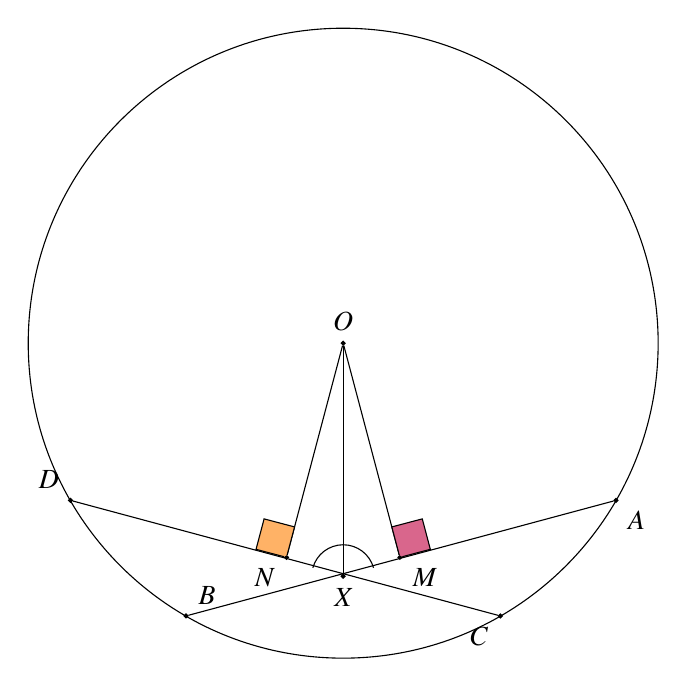
\begin{tikzpicture}
[scale=2,>=stealth,point/.style={draw,circle,fill = black,inner sep=0.5pt},]

%Triangle sides
\def\a{5}
\def\b{6}
\def\r{2}
%Coordinates of A
\def\pa{1.732}
\def\qa{0.998}
\def\pb{-1.732}
\def\qb{-0.998}
\def\mx{0.36}
\def\my{-1.36}
\draw (0,0) circle (2cm);
%Labeling points
\node (A) at (\pa,\qb)[point,label=below right:$A$] {};
\node (B) at (\qb, \pb)[point,label=above right:$B$] {};
\node (M) at (0.36,-1.36)[point,label=below right:$M$] {};
\node (N) at (-0.36,-1.36)[point,label=below left:$N$] {};
\node (X) at (0,-1.48)[point,label=below:$X$] {};

\node (C) at (\qa,\pb)[point,label=below left:$C$] {};
\node (D) at (\pb, \qb)[point,label=above left:$D$] {};
%\node (Y) at (\q, 0)[point,label=left:$Y$] {};

\node (O) at (0,0)[point,label=above:$O$]{};

%Drawing triangle ABC
\draw (A) --  (B);
\draw (X)-- (O);
\draw (C) --  (D);
\draw (N)-- (O);
\draw (M)-- (O);
%Drawing medians BE and CF
%\draw (D) -- (E);
%\draw (D) -- (F);
%\draw (O) -- (B);
%\draw (O) -- (C);
%Drawing EF
%\draw (E) -- (F);

%Labeling sides
%\node [right] at ($(A)!0.5!(E)$) {$\frac{b}{2}$};
%\node [right] at ($(C)!0.5!(E)$) {$\frac{b}{2}$};
%\node [left] at ($(B)!0.5!(F)$) {$\frac{c}{2}$};
%\node [left] at ($(A)!0.5!(F)$) {$\frac{c}{2}$};

%Angles
\tkzMarkRightAngle[fill=purple!60,size=.2](A,M,O)
\tkzMarkRightAngle[fill=orange!60,size=.2](O,N,D)
%\tkzMarkAngle[fill=green!60,size=.3](O,B,A)
%
\tkzMarkAngle[fill=red!60,size=.2](O,X,D)
\tkzMarkAngle[fill=green!60,size=.2](A,X,O)
%%
%\tkzMarkAngle[fill=yellow!60,size=.2](A,D,E)
%\tkzMarkAngle[fill=yellow!60,size=.2](A,O,B)
%%
%\tkzMarkAngle[fill=orange!60,size=.2](F,D,A)
%\tkzMarkAngle[fill=orange!60,size=.2](C,O,A)
%
%\tkzMarkAngle[fill=blue!60,size=.3](E,A,F)
\end{tikzpicture}
}
\caption{Circle by Latex-Tikz}
\label{fig:stepthreetex}	
\end{figure}

\item 
Two chords are said to be equal if their lengths are the same. The length of a chord is given by 2r$\sin{\frac{\theta}{2}}$, where $\vec{r}$ is the radius and  $\theta$ is the angle subtended by the chord at the center of the circle. Thus in a circle, equal chords subtend equal angles at the center.

\item Let us assume that the two equal chords $\vec{AB}$ and $\vec{CD}$ subtend equal angles of $\theta$ = 90$\degree$ at the center of the circle. $\theta_1$ and $\theta_2$ are the angles between x-axis and points $\vec{B}$ and $\vec{D}$ respectively.

%\begin{comment}
The values used for constructing the circle in both Python and \LaTeX{}-Tikz is in Table \ref{table:table1}:\\
\begin{table}[ht]
    \begin{center}
    	%%%%%%%%%%%%%%%%%%%%%%%%%%%%%%%%%%%%%%%%%%%%%%%%%%%%%%%%%%%%%%%%%%%%%%
%%                                                                  %%
%%  This is the header of a LaTeX2e file exported from Gnumeric.    %%
%%                                                                  %%
%%  This file can be compiled as it stands or included in another   %%
%%  LaTeX document. The table is based on the longtable package so  %%
%%  the longtable options (headers, footers...) can be set in the   %%
%%  preamble section below (see PRAMBLE).                           %%
%%                                                                  %%
%%  To include the file in another, the following two lines must be %%
%%  in the including file:                                          %%
%%        \def\inputGnumericTable{}                                 %%
%%  at the beginning of the file and:                               %%
%%        \input{name-of-this-file.tex}                             %%
%%  where the table is to be placed. Note also that the including   %%
%%  file must use the following packages for the table to be        %%
%%  rendered correctly:                                             %%
%%    \usepackage[latin1]{inputenc}                                 %%
%%    \usepackage{color}                                            %%
%%    \usepackage{array}                                            %%
%%    \usepackage{longtable}                                        %%
%%    \usepackage{calc}                                             %%
%%    \usepackage{multirow}                                         %%
%%    \usepackage{hhline}                                           %%
%%    \usepackage{ifthen}                                           %%
%%  optionally (for landscape tables embedded in another document): %%
%%    \usepackage{lscape}                                           %%
%%                                                                  %%
%%%%%%%%%%%%%%%%%%%%%%%%%%%%%%%%%%%%%%%%%%%%%%%%%%%%%%%%%%%%%%%%%%%%%%



%%  This section checks if we are begin input into another file or  %%
%%  the file will be compiled alone. First use a macro taken from   %%
%%  the TeXbook ex 7.7 (suggestion of Han-Wen Nienhuys).            %%
\def\ifundefined#1{\expandafter\ifx\csname#1\endcsname\relax}


%%  Check for the \def token for inputed files. If it is not        %%
%%  defined, the file will be processed as a standalone and the     %%
%%  preamble will be used.                                          %%
\ifundefined{inputGnumericTable}

%%  We must be able to close or not the document at the end.        %%
	\def\gnumericTableEnd{\end{document}}


%%%%%%%%%%%%%%%%%%%%%%%%%%%%%%%%%%%%%%%%%%%%%%%%%%%%%%%%%%%%%%%%%%%%%%
%%                                                                  %%
%%  This is the PREAMBLE. Change these values to get the right      %%
%%  paper size and other niceties.                                  %%
%%                                                                  %%
%%%%%%%%%%%%%%%%%%%%%%%%%%%%%%%%%%%%%%%%%%%%%%%%%%%%%%%%%%%%%%%%%%%%%%

	\documentclass[12pt%
			  %,landscape%
                    ]{report}
       \usepackage[latin1]{inputenc}
       \usepackage{fullpage}
       \usepackage{color}
       \usepackage{array}
       \usepackage{longtable}
       \usepackage{calc}
       \usepackage{multirow}
       \usepackage{hhline}
       \usepackage{ifthen}

	\begin{document}


%%  End of the preamble for the standalone. The next section is for %%
%%  documents which are included into other LaTeX2e files.          %%
\else

%%  We are not a stand alone document. For a regular table, we will %%
%%  have no preamble and only define the closing to mean nothing.   %%
    \def\gnumericTableEnd{}

%%  If we want landscape mode in an embedded document, comment out  %%
%%  the line above and uncomment the two below. The table will      %%
%%  begin on a new page and run in landscape mode.                  %%
%       \def\gnumericTableEnd{\end{landscape}}
%       \begin{landscape}


%%  End of the else clause for this file being \input.              %%
\fi

%%%%%%%%%%%%%%%%%%%%%%%%%%%%%%%%%%%%%%%%%%%%%%%%%%%%%%%%%%%%%%%%%%%%%%
%%                                                                  %%
%%  The rest is the gnumeric table, except for the closing          %%
%%  statement. Changes below will alter the table's appearance.     %%
%%                                                                  %%
%%%%%%%%%%%%%%%%%%%%%%%%%%%%%%%%%%%%%%%%%%%%%%%%%%%%%%%%%%%%%%%%%%%%%%

\providecommand{\gnumericmathit}[1]{#1} 
%%  Uncomment the next line if you would like your numbers to be in %%
%%  italics if they are italizised in the gnumeric table.           %%
%\renewcommand{\gnumericmathit}[1]{\mathit{#1}}
\providecommand{\gnumericPB}[1]%
{\let\gnumericTemp=\\#1\let\\=\gnumericTemp\hspace{0pt}}
 \ifundefined{gnumericTableWidthDefined}
        \newlength{\gnumericTableWidth}
        \newlength{\gnumericTableWidthComplete}
        \newlength{\gnumericMultiRowLength}
        \global\def\gnumericTableWidthDefined{}
 \fi
%% The following setting protects this code from babel shorthands.  %%
 \ifthenelse{\isundefined{\languageshorthands}}{}{\languageshorthands{english}}
%%  The default table format retains the relative column widths of  %%
%%  gnumeric. They can easily be changed to c, r or l. In that case %%
%%  you may want to comment out the next line and uncomment the one %%
%%  thereafter                                                      %%
\providecommand\gnumbox{\makebox[0pt]}
%%\providecommand\gnumbox[1][]{\makebox}

%% to adjust positions in multirow situations                       %%
\setlength{\bigstrutjot}{\jot}
\setlength{\extrarowheight}{\doublerulesep}

%%  The \setlongtables command keeps column widths the same across  %%
%%  pages. Simply comment out next line for varying column widths.  %%
\setlongtables

\setlength\gnumericTableWidth{%
	70pt+%
	70pt+%
0pt}
\def\gumericNumCols{2}
\setlength\gnumericTableWidthComplete{\gnumericTableWidth+%
         \tabcolsep*\gumericNumCols*2+\arrayrulewidth*\gumericNumCols}
\ifthenelse{\lengthtest{\gnumericTableWidthComplete > \linewidth}}%
         {\def\gnumericScale{\ratio{\linewidth-%
                        \tabcolsep*\gumericNumCols*2-%
                        \arrayrulewidth*\gumericNumCols}%
{\gnumericTableWidth}}}%
{\def\gnumericScale{1}}

%%%%%%%%%%%%%%%%%%%%%%%%%%%%%%%%%%%%%%%%%%%%%%%%%%%%%%%%%%%%%%%%%%%%%%
%%                                                                  %%
%% The following are the widths of the various columns. We are      %%
%% defining them here because then they are easier to change.       %%
%% Depending on the cell formats we may use them more than once.    %%
%%                                                                  %%
%%%%%%%%%%%%%%%%%%%%%%%%%%%%%%%%%%%%%%%%%%%%%%%%%%%%%%%%%%%%%%%%%%%%%%

\ifthenelse{\isundefined{\gnumericColA}}{\newlength{\gnumericColA}}{}\settowidth{\gnumericColA}{\begin{tabular}{@{}p{70pt*\gnumericScale}@{}}x\end{tabular}}
\ifthenelse{\isundefined{\gnumericColB}}{\newlength{\gnumericColB}}{}\settowidth{\gnumericColB}{\begin{tabular}{@{}p{70pt*\gnumericScale}@{}}x\end{tabular}}

\begin{tabular}[c]{%
	b{\gnumericColA}%
	b{\gnumericColB}%
	}

%%%%%%%%%%%%%%%%%%%%%%%%%%%%%%%%%%%%%%%%%%%%%%%%%%%%%%%%%%%%%%%%%%%%%%
%%  The longtable options. (Caption, headers... see Goosens, p.124) %%
%	\caption{The Table Caption.}             \\	%
% \hline	% Across the top of the table.
%%  The rest of these options are table rows which are placed on    %%
%%  the first, last or every page. Use \multicolumn if you want.    %%

%%  Header for the first page.                                      %%
%	\multicolumn{2}{c}{The First Header} \\ \hline 
%	\multicolumn{1}{c}{colTag}	%Column 1
%	&\multicolumn{1}{c}{colTag}	\\ \hline %Last column
%	\endfirsthead

%%  The running header definition.                                  %%
%	\hline
%	\multicolumn{2}{l}{\ldots\small\slshape continued} \\ \hline
%	\multicolumn{1}{c}{colTag}	%Column 1
%	&\multicolumn{1}{c}{colTag}	\\ \hline %Last column
%	\endhead

%%  The running footer definition.                                  %%
%	\hline
%	\multicolumn{2}{r}{\small\slshape continued\ldots} \\
%	\endfoot

%%  The ending footer definition.                                   %%
%	\multicolumn{2}{c}{That's all folks} \\ \hline 
%	\endlastfoot
%%%%%%%%%%%%%%%%%%%%%%%%%%%%%%%%%%%%%%%%%%%%%%%%%%%%%%%%%%%%%%%%%%%%%%

\hhline{|--}
	 \multicolumn{2}{|p{	\gnumericColA+%
	\gnumericColB+%
	\tabcolsep*2*1}|}%
	{\gnumericPB{\centering}\gnumbox{\textbf{Initial Input Values}}}
\\
\hhline{|-|-|}
	 \multicolumn{1}{|p{\gnumericColA}|}%
	{\gnumericPB{\centering}\gnumbox{\textbf{Parameters}}}
	&\multicolumn{1}{p{\gnumericColB}|}%
	{\gnumericPB{\centering}\gnumbox{\textbf{Values}}}
\\
\hhline{|--|}
	 \multicolumn{1}{|p{\gnumericColA}|}%
	{\gnumericPB{\centering}\gnumbox{\textbf{r}}}
	&\multicolumn{1}{p{\gnumericColB}|}%
	{\gnumericPB{\centering}\gnumbox{\textbf{2}}}
\\
\hhline{|--|}
	 \multicolumn{1}{|p{\gnumericColA}|}%
	{\gnumericPB{\centering}\gnumbox{\textbf{$\theta$}}}
	&\multicolumn{1}{p{\gnumericColB}|}%
	{\gnumericPB{\centering}\gnumbox{\textbf{90$\degree$}}}
\\
\hhline{|--|}
	 \multicolumn{1}{|p{\gnumericColA}|}%
	{\gnumericPB{\centering}\gnumbox{\textbf{$\theta_1$}}}
	&\multicolumn{1}{p{\gnumericColB}|}%
	{\gnumericPB{\centering}\gnumbox{\textbf{-120$\degree$}}}
\\
\hhline{|--|}
	 \multicolumn{1}{|p{\gnumericColA}|}%
	{\gnumericPB{\centering}\gnumbox{\textbf{$\theta_2$}}}
	&\multicolumn{1}{p{\gnumericColB}|}%
	{\gnumericPB{\centering}\gnumbox{\textbf{210$\degree$}}}
\\
\hhline{|-|-|}
\end{tabular}

\ifthenelse{\isundefined{\languageshorthands}}{}{\languageshorthands{\languagename}}
\gnumericTableEnd

  \caption{To construct circle O}
   \label{table:table1}
   \end{center}	
\end{table}
%\end{comment}


\item Finding the coordinates of various points of Fig. \ref{fig:stepthreetex}, let 
\quad $ \vec{O}= \begin{pmatrix}0\\0\end{pmatrix}$
%  \quad $\vec{A}=\begin{pmatrix}r\cos{\big(\theta _1 + \frac{\pi}{2}\big)}\\r\sin{\big{\theta _1 + \frac{\pi}{2}\big)}\end{pmatrix}$

  \quad $ \vec{B}= \begin{pmatrix}r\cos{\theta _1}\\r\sin{\theta _1}\end{pmatrix}$
  \quad $\vec{A}=\begin{pmatrix}r\cos{\big(\theta _1 + \theta\big)}\\r\sin{\big(\theta _1 + \theta\big)}\end{pmatrix}$

  \quad $ \vec{D}= \begin{pmatrix}r\cos{\theta _2}\\r\sin{\theta _2}\end{pmatrix}$
  \quad $\vec{C}=\begin{pmatrix}r\cos{\big(\theta _2 + \theta\big)}\\r\sin{\big(\theta _2 + \theta\big)}\end{pmatrix}$

\item As $\vec{OM} and \vec{ON}$ are the perpendiculars from the center of the circle to the chord,which are the midpoints of $\vec{AB}$ and $\vec{CD}$, and are hence represented as:\\
  \quad $ \vec{M}$ = $\frac{\vec{A+B}}{2}$\quad
  \quad $ \vec{N}$ = $\frac{\vec{C+D}}{2}$\\ 



%\begin{comment}
The derived values used is in Table \ref{table:table2}:\\
\begin{table}[ht]
    \begin{center}
    	%%%%%%%%%%%%%%%%%%%%%%%%%%%%%%%%%%%%%%%%%%%%%%%%%%%%%%%%%%%%%%%%%%%%%%
%%                                                                  %%
%%  This is the header of a LaTeX2e file exported from Gnumeric.    %%
%%                                                                  %%
%%  This file can be compiled as it stands or included in another   %%
%%  LaTeX document. The table is based on the longtable package so  %%
%%  the longtable options (headers, footers...) can be set in the   %%
%%  preamble section below (see PRAMBLE).                           %%
%%                                                                  %%
%%  To include the file in another, the following two lines must be %%
%%  in the including file:                                          %%
%%        \def\inputGnumericTable{}                                 %%
%%  at the beginning of the file and:                               %%
%%        \input{name-of-this-file.tex}                             %%
%%  where the table is to be placed. Note also that the including   %%
%%  file must use the following packages for the table to be        %%
%%  rendered correctly:                                             %%
%%    \usepackage[latin1]{inputenc}                                 %%
%%    \usepackage{color}                                            %%
%%    \usepackage{array}                                            %%
%%    \usepackage{longtable}                                        %%
%%    \usepackage{calc}                                             %%
%%    \usepackage{multirow}                                         %%
%%    \usepackage{hhline}                                           %%
%%    \usepackage{ifthen}                                           %%
%%  optionally (for landscape tables embedded in another document): %%
%%    \usepackage{lscape}                                           %%
%%                                                                  %%
%%%%%%%%%%%%%%%%%%%%%%%%%%%%%%%%%%%%%%%%%%%%%%%%%%%%%%%%%%%%%%%%%%%%%%



%%  This section checks if we are begin input into another file or  %%
%%  the file will be compiled alone. First use a macro taken from   %%
%%  the TeXbook ex 7.7 (suggestion of Han-Wen Nienhuys).            %%
\def\ifundefined#1{\expandafter\ifx\csname#1\endcsname\relax}


%%  Check for the \def token for inputed files. If it is not        %%
%%  defined, the file will be processed as a standalone and the     %%
%%  preamble will be used.                                          %%
\ifundefined{inputGnumericTable}

%%  We must be able to close or not the document at the end.        %%
	\def\gnumericTableEnd{\end{document}}


%%%%%%%%%%%%%%%%%%%%%%%%%%%%%%%%%%%%%%%%%%%%%%%%%%%%%%%%%%%%%%%%%%%%%%
%%                                                                  %%
%%  This is the PREAMBLE. Change these values to get the right      %%
%%  paper size and other niceties.                                  %%
%%                                                                  %%
%%%%%%%%%%%%%%%%%%%%%%%%%%%%%%%%%%%%%%%%%%%%%%%%%%%%%%%%%%%%%%%%%%%%%%

	\documentclass[12pt%
			  %,landscape%
                    ]{report}
       \usepackage[latin1]{inputenc}
       \usepackage{fullpage}
       \usepackage{color}
       \usepackage{array}
       \usepackage{longtable}
       \usepackage{calc}
       \usepackage{multirow}
       \usepackage{hhline}
       \usepackage{ifthen}

	\begin{document}


%%  End of the preamble for the standalone. The next section is for %%
%%  documents which are included into other LaTeX2e files.          %%
\else

%%  We are not a stand alone document. For a regular table, we will %%
%%  have no preamble and only define the closing to mean nothing.   %%
    \def\gnumericTableEnd{}

%%  If we want landscape mode in an embedded document, comment out  %%
%%  the line above and uncomment the two below. The table will      %%
%%  begin on a new page and run in landscape mode.                  %%
%       \def\gnumericTableEnd{\end{landscape}}
%       \begin{landscape}


%%  End of the else clause for this file being \input.              %%
\fi

%%%%%%%%%%%%%%%%%%%%%%%%%%%%%%%%%%%%%%%%%%%%%%%%%%%%%%%%%%%%%%%%%%%%%%
%%                                                                  %%
%%  The rest is the gnumeric table, except for the closing          %%
%%  statement. Changes below will alter the table's appearance.     %%
%%                                                                  %%
%%%%%%%%%%%%%%%%%%%%%%%%%%%%%%%%%%%%%%%%%%%%%%%%%%%%%%%%%%%%%%%%%%%%%%

\providecommand{\gnumericmathit}[1]{#1} 
%%  Uncomment the next line if you would like your numbers to be in %%
%%  italics if they are italizised in the gnumeric table.           %%
%\renewcommand{\gnumericmathit}[1]{\mathit{#1}}
\providecommand{\gnumericPB}[1]%
{\let\gnumericTemp=\\#1\let\\=\gnumericTemp\hspace{0pt}}
 \ifundefined{gnumericTableWidthDefined}
        \newlength{\gnumericTableWidth}
        \newlength{\gnumericTableWidthComplete}
        \newlength{\gnumericMultiRowLength}
        \global\def\gnumericTableWidthDefined{}
 \fi
%% The following setting protects this code from babel shorthands.  %%
 \ifthenelse{\isundefined{\languageshorthands}}{}{\languageshorthands{english}}
%%  The default table format retains the relative column widths of  %%
%%  gnumeric. They can easily be changed to c, r or l. In that case %%
%%  you may want to comment out the next line and uncomment the one %%
%%  thereafter                                                      %%
\providecommand\gnumbox{\makebox[0pt]}
%%\providecommand\gnumbox[1][]{\makebox}

%% to adjust positions in multirow situations                       %%
\setlength{\bigstrutjot}{\jot}
\setlength{\extrarowheight}{\doublerulesep}

%%  The \setlongtables command keeps column widths the same across  %%
%%  pages. Simply comment out next line for varying column widths.  %%
\setlongtables

\setlength\gnumericTableWidth{%
	73pt+%
	67pt+%
0pt}
\def\gumericNumCols{2}
\setlength\gnumericTableWidthComplete{\gnumericTableWidth+%
         \tabcolsep*\gumericNumCols*2+\arrayrulewidth*\gumericNumCols}
\ifthenelse{\lengthtest{\gnumericTableWidthComplete > \linewidth}}%
         {\def\gnumericScale{\ratio{\linewidth-%
                        \tabcolsep*\gumericNumCols*2-%
                        \arrayrulewidth*\gumericNumCols}%
{\gnumericTableWidth}}}%
{\def\gnumericScale{1}}

%%%%%%%%%%%%%%%%%%%%%%%%%%%%%%%%%%%%%%%%%%%%%%%%%%%%%%%%%%%%%%%%%%%%%%
%%                                                                  %%
%% The following are the widths of the various columns. We are      %%
%% defining them here because then they are easier to change.       %%
%% Depending on the cell formats we may use them more than once.    %%
%%                                                                  %%
%%%%%%%%%%%%%%%%%%%%%%%%%%%%%%%%%%%%%%%%%%%%%%%%%%%%%%%%%%%%%%%%%%%%%%

\ifthenelse{\isundefined{\gnumericColA}}{\newlength{\gnumericColA}}{}\settowidth{\gnumericColA}{\begin{tabular}{@{}p{73pt*\gnumericScale}@{}}x\end{tabular}}
\ifthenelse{\isundefined{\gnumericColB}}{\newlength{\gnumericColB}}{}\settowidth{\gnumericColB}{\begin{tabular}{@{}p{67pt*\gnumericScale}@{}}x\end{tabular}}

\begin{tabular}[c]{%
	b{\gnumericColA}%
	b{\gnumericColB}%
	}

%%%%%%%%%%%%%%%%%%%%%%%%%%%%%%%%%%%%%%%%%%%%%%%%%%%%%%%%%%%%%%%%%%%%%%
%%  The longtable options. (Caption, headers... see Goosens, p.124) %%
%	\caption{The Table Caption.}             \\	%
% \hline	% Across the top of the table.
%%  The rest of these options are table rows which are placed on    %%
%%  the first, last or every page. Use \multicolumn if you want.    %%

%%  Header for the first page.                                      %%
%	\multicolumn{2}{c}{The First Header} \\ \hline 
%	\multicolumn{1}{c}{colTag}	%Column 1
%	&\multicolumn{1}{c}{colTag}	\\ \hline %Last column
%	\endfirsthead

%%  The running header definition.                                  %%
%	\hline
%	\multicolumn{2}{l}{\ldots\small\slshape continued} \\ \hline
%	\multicolumn{1}{c}{colTag}	%Column 1
%	&\multicolumn{1}{c}{colTag}	\\ \hline %Last column
%	\endhead

%%  The running footer definition.                                  %%
%	\hline
%	\multicolumn{2}{r}{\small\slshape continued\ldots} \\
%	\endfoot

%%  The ending footer definition.                                   %%
%	\multicolumn{2}{c}{That's all folks} \\ \hline 
%	\endlastfoot
%%%%%%%%%%%%%%%%%%%%%%%%%%%%%%%%%%%%%%%%%%%%%%%%%%%%%%%%%%%%%%%%%%%%%%

\hhline{|--}
	 \multicolumn{2}{|p{	\gnumericColA+%
	\gnumericColB+%
	\tabcolsep*2*1}|}%
	{\gnumericPB{\centering}\gnumbox{\textbf{Derived Values}}}
\\
\hhline{|-|-|}
	 \multicolumn{1}{|p{\gnumericColA}|}%
	{\gnumericPB{\centering}\gnumbox{\textbf{Parameter}}}
	&\multicolumn{1}{p{\gnumericColB}|}%
	{\gnumericPB{\centering}\gnumbox{\textbf{Value}}}
\\
\hhline{|--|}
	 \multicolumn{1}{|p{\gnumericColA}|}%
	{\gnumericPB{\centering}\gnumbox{\textbf{ChordLength}}}
	&\multicolumn{1}{p{\gnumericColB}|}%
	{\gnumericPB{\centering}\gnumbox{\textbf{2.82}}}
\\
\hhline{|--|}
	 \multicolumn{1}{|p{\gnumericColA}|}%
	{\gnumericPB{\centering}\gnumbox{\textbf{A}}}
	&\multicolumn{1}{p{\gnumericColB}|}%
	{\gnumericPB{\centering}\gnumbox{\textbf{$\myvec{1.73\\-0.99}$}}}
\\
\hhline{|--|}
	 \multicolumn{1}{|p{\gnumericColA}|}%
	{\gnumericPB{\centering}\gnumbox{\textbf{B}}}
	&\multicolumn{1}{p{\gnumericColB}|}%
	{\gnumericPB{\centering}\gnumbox{\textbf{$\myvec{-0.99\\-1.73}$}}}
\\
\hhline{|--|}
	 \multicolumn{1}{|p{\gnumericColA}|}%
	{\gnumericPB{\centering}\gnumbox{\textbf{C }}}
	&\multicolumn{1}{p{\gnumericColB}|}%
	{\gnumericPB{\centering}\gnumbox{\textbf{$\myvec{0.99\\-1.73}$}}}
\\
\hhline{|--|}
	 \multicolumn{1}{|p{\gnumericColA}|}%
	{\gnumericPB{\centering}\gnumbox{\textbf{D }}}
	&\multicolumn{1}{p{\gnumericColB}|}%
	{\gnumericPB{\centering}\gnumbox{\textbf{$\myvec{-1.73\\-0.99}$}}}
\\
\hhline{|--|}
	 \multicolumn{1}{|p{\gnumericColA}|}%
	{\gnumericPB{\centering}\gnumbox{\textbf{M}}}
	&\multicolumn{1}{p{\gnumericColB}|}%
	{\gnumericPB{\centering}\gnumbox{\textbf{$\myvec{0.36\\-1.36}$}}}
\\
\hhline{|--|}
	 \multicolumn{1}{|p{\gnumericColA}|}%
	{\gnumericPB{\centering}\gnumbox{\textbf{N}}}
	&\multicolumn{1}{p{\gnumericColB}|}%
	{\gnumericPB{\centering}\gnumbox{\textbf{$\myvec{-0.36\\-1.36}$}}}
\\
\hhline{|--|}
	 \multicolumn{1}{|p{\gnumericColA}|}%
	{\gnumericPB{\centering}\gnumbox{\textbf{X}}}
	&\multicolumn{1}{p{\gnumericColB}|}%
	{\gnumericPB{\centering}\gnumbox{\textbf{$\myvec{0\\-1.45}$}}}
\\

\hhline{|-|-|}
\end{tabular}

\ifthenelse{\isundefined{\languageshorthands}}{}{\languageshorthands{\languagename}}
\gnumericTableEnd

  \caption{To construct circle O}
   \label{table:table2}
   \end{center}	
\end{table}
%\end{comment}

















\end{enumerate}

\subsubsection*{To Show:}    We need to prove that $\angle{OXD}$ = $\angle{AXO}$.\\

\section{\textbf{Solution}}
\renewcommand{\vec}[1]{\mathbf{#1}}
 \begin{enumerate}


\item First we need to show that a perpendicular from the center of a circle to a chord bisects the chord.\\

Take a circle C of radius $\vec{r}$=2cm, whose center is $\vec{O}$ such that $ \vec{O}$= $\begin{pmatrix}0\\0\end{pmatrix}$. 
$\vec{AB}$ is a chord such that $\vec{OX} \perp \vec{AB}$. We need to show that $\vec{AX}$ = $\vec{BX}$.
\newline
 
\begin{enumerate}
	\item $\triangle OAX \cong \triangle OBX $by RHS rule as: 
	\begin{enumerate}
	\item $\angle{OXA} = \angle{OXB} $ \quad \{90\degree\}
	\item $\vec{OA} = \vec{OB}$ \quad \{radius of the circle\}
	\item $\vec{OX} = \vec{OX}$ \quad \{Common\}
	\end{enumerate}
\end{enumerate}
	Therefore $\vec{AX} = \vec{BX}$\\
	Hence the perpendicular from the center of a circle to a chord bisects the chord.

  
\begin{figure}[!ht]
\centering
\resizebox{\columnwidth}{!}{
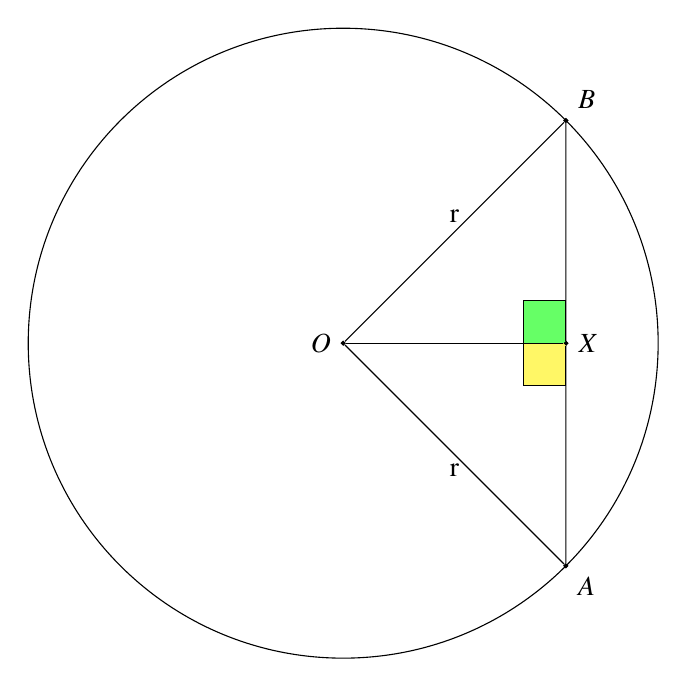
\begin{tikzpicture}
[scale=2,>=stealth,point/.style={draw,circle,fill = black,inner sep=0.5pt},]

%Triangle sides
\def\a{5}
\def\b{6}
\def\r{2}
%Coordinates of A
\def\p{1.414}
\def\q{-1.414}
\draw (0,0) circle (2cm);
%Labeling points
\node (A) at (\p,\q)[point,label=below right:$A$] {};
\node (B) at (\p, \p)[point,label=above right:$B$] {};
\node (X) at (\p, 0)[point,label=right:$X$] {};
\node (O) at (0,0)[point,label=left:$O$]{};
%Foot of median

%\node (D) at ($(A)!0.5!(O)$)[point,label=below:$D$] {};
%\node (E) at ($(A)!0.5!(B)$)[point,label=left:$E$] {};
%\node (F) at ($(C)!0.5!(A)$)[point,label=right:$F$] {};

%Drawing triangle ABC
\draw (A) --  (B) -- node[above] {$\textrm{r}$} (O) -- node[below] {$\textrm{r}$} (A);
\draw (X)-- (O);
%Drawing medians BE and CF
%\draw (D) -- (E);
%\draw (D) -- (F);
%\draw (O) -- (B);
%\draw (O) -- (C);
%Drawing EF
%\draw (E) -- (F);

%Labeling sides
%\node [right] at ($(A)!0.5!(E)$) {$\frac{b}{2}$};
%\node [right] at ($(C)!0.5!(E)$) {$\frac{b}{2}$};
%\node [left] at ($(B)!0.5!(F)$) {$\frac{c}{2}$};
%\node [left] at ($(A)!0.5!(F)$) {$\frac{c}{2}$};

%Angles
\tkzMarkRightAngle[fill=green!60,size=.27](O,X,B)
\tkzMarkRightAngle[fill=yellow!60,size=.27](O,X,A)
%\tkzMarkAngle[fill=green!60,size=.3](O,B,A)
%
%\tkzMarkAngle[fill=red!60,size=.7](A,F,D)
%\tkzMarkAngle[fill=red!60,size=.7](A,C,O)
%%
%\tkzMarkAngle[fill=yellow!60,size=.2](A,D,E)
%\tkzMarkAngle[fill=yellow!60,size=.2](A,O,B)
%%
%\tkzMarkAngle[fill=orange!60,size=.2](F,D,A)
%\tkzMarkAngle[fill=orange!60,size=.2](C,O,A)
%
%\tkzMarkAngle[fill=blue!60,size=.3](E,A,F)
\end{tikzpicture}
}
\caption{Circle by Latex-Tikz}
\label{fig:stepone}	
\end{figure}
\end{enumerate}




\item Next we need to show that equal chords of a circle are equidistant from the center.\\

Take a circle C of radius $\vec{r}$=2cm, whose center is $\vec{O}$ such that $ \vec{O}$= $\begin{pmatrix}0\\0\end{pmatrix}$. 
$\vec{AB}$ and $\vec{CD}$ are chords such that $\vec{OX} \perp \vec{AB}$ and $\vec{OY} \perp \vec{CD}$. We need to show that $\vec{OX}$ = $\vec{OY}$.
\newline
 

\begin{enumerate}
	
	\item Since $\vec{OX} \perp \vec{AB}$, $\vec{AX} =  \vec{BX} = \frac{\vec{AB}}{2}$ \{perpendicular from the center of a circle to a chord bisects the chord. \}\\
	Similarly $\vec{CY} =  \vec{DY} = \frac{\vec{CY}}{2}$\\
	\item As $\vec{AB} =  \vec{CD}$\\
	$\frac{\vec{AB}}{2} = \frac{\vec{CD}}{2}$\\
	Hence $\vec{AX} =  \vec{CY}$\\
	
	\item In $\triangle AOX$ and $\triangle COY $\\
	
	\begin{enumerate}
	\item $\angle{OXA} = \angle{OYC} $ \quad \{90\degree\}
	\item $\vec{OA} = \vec{OC}$ \quad \{radius of the circle\}
	\item $\vec{AX} = \vec{CY}$ \quad \{Common\}
	\end{enumerate}
	Hence  $\triangle AOX \cong \triangle COY $by RHS rule.\\
	Therefore, $\vec{OX}=\vec{OY}$
\end{enumerate}
	Hence the equal chords of a circle are equidistant from the center.\\

  
\begin{figure}[!ht]
\centering
\resizebox{\columnwidth}{!}{
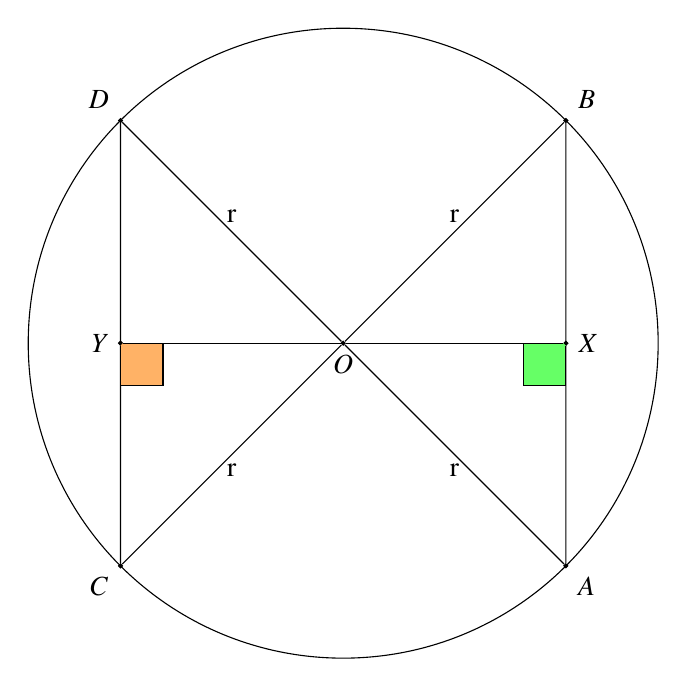
\begin{tikzpicture}
[scale=2,>=stealth,point/.style={draw,circle,fill = black,inner sep=0.5pt},]

%Triangle sides
\def\a{5}
\def\b{6}
\def\r{2}
%Coordinates of A
\def\p{1.414}
\def\q{-1.414}
\draw (0,0) circle (2cm);
%Labeling points
\node (A) at (\p,\q)[point,label=below right:$A$] {};
\node (B) at (\p, \p)[point,label=above right:$B$] {};
\node (X) at (\p, 0)[point,label=right:$X$] {};

\node (C) at (\q,\q)[point,label=below left:$C$] {};
\node (D) at (\q, \p)[point,label=above left:$D$] {};
\node (Y) at (\q, 0)[point,label=left:$Y$] {};

\node (O) at (0,0)[point,label=below:$O$]{};

%Drawing triangle ABC
\draw (A) --  (B) -- node[above] {$\textrm{r}$} (O) -- node[below] {$\textrm{r}$} (A);
\draw (X)-- (O);
\draw (C) --  (D) -- node[above] {$\textrm{r}$} (O) -- node[below] {$\textrm{r}$} (C);
\draw (Y)-- (O);
%Drawing medians BE and CF
%\draw (D) -- (E);
%\draw (D) -- (F);
%\draw (O) -- (B);
%\draw (O) -- (C);
%Drawing EF
%\draw (E) -- (F);

%Labeling sides
%\node [right] at ($(A)!0.5!(E)$) {$\frac{b}{2}$};
%\node [right] at ($(C)!0.5!(E)$) {$\frac{b}{2}$};
%\node [left] at ($(B)!0.5!(F)$) {$\frac{c}{2}$};
%\node [left] at ($(A)!0.5!(F)$) {$\frac{c}{2}$};

%Angles
\tkzMarkRightAngle[fill=green!60,size=.27](O,X,A)
\tkzMarkRightAngle[fill=orange!60,size=.27](O,Y,C)
%\tkzMarkAngle[fill=green!60,size=.3](O,B,A)
%
%\tkzMarkAngle[fill=red!60,size=.7](A,F,D)
%\tkzMarkAngle[fill=red!60,size=.7](A,C,O)
%%
%\tkzMarkAngle[fill=yellow!60,size=.2](A,D,E)
%\tkzMarkAngle[fill=yellow!60,size=.2](A,O,B)
%%
%\tkzMarkAngle[fill=orange!60,size=.2](F,D,A)
%\tkzMarkAngle[fill=orange!60,size=.2](C,O,A)
%
%\tkzMarkAngle[fill=blue!60,size=.3](E,A,F)
\end{tikzpicture}
}
\caption{Circle by Latex-Tikz}
\label{fig:steptwo}	
\end{figure}
\end{enumerate}






\end{document}
